\chapter{Estat de l'art}
\label{cap:estat-de-l-art}

Aquest capítol té per objectiu resumir i ordenar de forma estructurada la
recerca inicial que s'ha fet per a aquest projecte. Només es posarà èmfasi en
les parts rellevants per el projecte, però sempre s'inclourà alguna referència
per a complementar o ampliar algun concepte.

\section{\acro{Usb}}

Sent la connexió \acro{usb} un dels objectius més cèntrics d'aquest treball de
fi de grau, s'ha iniciat la recerca aquest cantó. No només s'ha escollit usar
aquest estàndard per la seva compatibilitat
i facilitats que proporciona a l'usuari, sinó que també hi havia un interès
personal en entendre aquest protocol.

El \acro{usb}, que significa \est{Universal Serial Bus} en anglès, és un
estàndard de comunicació que permet la connexió, intercanvi i transferència de
dades entre dispositius electrònics com ara ordinadors, telèfons mòbils, i
impressores. Aquesta tecnologia utilitza uns connectors estàndards que son
àmpliament reconeguts per la seva facilitat d'ús i versatilitat en una àmplia
gamma d'aplicacions. Els dispositius USB poden transmetre dades a diferents
velocitats, des de velocitats molt baixes fins a velocitats molt altes,
i són compatibles amb una gran varietat de sistemes operatius i plataformes
de hardware \cite{Axelson2015USB}.

\subsection{Arquitectura}

L'arquitectura d'\acro{usb} és de tipus mestre-esclau, on el mestre sol ser
l'ordinador i l'esclau el dispositiu que es connecta. Com es veurà a l'Apartat
\ref{sec:usb_versions}, s'acabarà utilitzant la versió \acro{usb2}. Per
evitar fer molt extens aquest document, només es detallarà l'arquitectura
d'aquesta versió.

\subsubsection*{Aspectes físics}

No es detallarà molt el baix nivell ja que s'utilitzarà llibreries que
compleixen l'estàndard des d'un nivell més alt. Tanmateix, s'ha trobat
interessant fer una pinzellada de l'estàndard.

El connector \acro{usb2} està composat de 4 cables: \acro{5v}, \acro{gnd},
\acro{d+} i \acro{d-}. La funció del cable de \acro{5v} és alimentar el
dispositiu, amb una intensitat de fins a \SI{500}{\milli\ampere}. Aquestes
prestacions de corrent resulten ser suficients per a la major part dels
dispositius que compleixen l'estàndard. Sabent que \acro{gnd} és el cable
necessari per a tancar els circuits, només queda \acro{d+} i \acro{d-} per
a enviar dades.

Contràriament al que un podria pensar, el flux de dades (i electricitat) no
està predefinit: en un moment pot ser l'ordinador que utilitzi els dos cables
per a transmetre dades al dispositiu, i en un altre pot ser a l'inrevés. De fet,
els dos cables envien sempre el mateix, però invertit. D'aquesta forma es pot
detectar i corregir interferències molt més fàcilment, ja que aquestes solen
afectar per igual als dos cables (degut a la seva proximitat dins del
connector).

És important tenir en compte que la tensió d'operació de l'estàndard \acro{usb2}
és de \SI{3.3}{\volt}, encara que la tensió que proporciona el cable
d'alimentació sigui de \SI{5}{\volt}. Aquest detall serà molt important de cara
al disseny del dispositiu, ja que implicarà, molt probablement, l'ús de dos
díodes Zener a l'entrada de les línies de transmissió de dades.

\subsubsection*{Aspectes de baix nivell}

Tal i com s'ha comentat en l'apartat anterior, el canal de transmissió que
proporciona l'estàndard és unidireccional o \est{half-duplex}. En aquest
apartat es defineixen els tres tipus de transaccions.

Una transacció és un seguit d'intercanvi de dades entre l'ordinador i el
dispositiu. Totes s'inicien des de l'ordinador, encara que el paquet que es
vulgui enviar sigui en sentit invers. No s'entra en detall sobre el protocol
de connexió ja que no té importància per a aquest detall.

Existeixen tres tipus de transaccions:
\begin{itemize}
    \item Les transaccions \est{OUT} serveixen per a enviar paquets de
    l'ordinador al dispositiu.
    \item Les transaccions \est{IN} serveixen per a enviar paquets del
    dispositiu a l'ordinador. A diferència del tipus anterior, aquesta
    transacció no la inicia qui vol enviar el paquet. Per a poder
    solventar aquesta complicació existeix el següent tipus.
    \item Les transaccions de control serveixen per a poder esbrinar quan el
    dispositiu necessita enviar dades, pactar velocitats de transmissió, entre
    d'altres. La transacció de control més important és la \est{SETUP},
    que serveix per a intercanviar informació inicial entre els dispositius. Més
    endavant es veuran els tiups de dades que s'intercanvien inicialment.
\end{itemize}

L'important d'aquest apartat és tenir present que les transaccions \est{IN} i
\est{OUT} es van dissenyar per a mantenir un intercanvi de dades constant,
mentre que les transaccions de control, fora de l'etapa de \est{SETUP}, estan
més pensades per a petits intercanvis de dades, i més irregulars. Més endavant
resultarà aquesta informació important per a entendre la implementació del
dispositiu.

\subsubsection*{Metadades}

Durant els intercanvis inicials, durant l'etapa \est{SETUP}, el dispositiu
comparteix certes metadades a l'ordinador, cosa que el permet identificar-se,
i descriure les especificacions necessàries. Un dels avantatges més visibles
d'aquest procés invisible és la funcionalitat \est{plug\&play}, que evita
insta\l.lar programari per a cada nou dispositiu que es connecta.

Dos codis molt importants en aquest procés són el \acro{vid} i el \acro{pid},
acrònims de \est{Vendor ID} i \est{Product ID}. El \acro{vid} identifica
l'organisme que ha emès el dispositiu, i el \acro{pid} identifica el producte.
Cal tenir present que aquests dos codis son idèntics per a tots els dispositius
que es produeixin, pel que no té res a veure amb un número de sèrie. El motiu
pel que es divideix el codi en dos nombres diferents recau en la forma en la
que s'assignen als dispositius, tal i com s'explicarà més endavant. Tanmateix,
a efectes tècnics es considera com un únic nombre.

Aquests codis tenen per objectiu que l'ordinador pugui identificar el tipus de
dispositiu que s'ha connectat. Un dels usos principals d'aquesta funcionalitat
és la creació de regles \est{udev}, que en els sistemes de Linux assignen
\est{drivers} en funció dels codis anteriorment esmentats.

Una altra metadada que s'intercanvia a l'inici de la connexió és la classe
de dispositiu. Aquesta pot diferenciar entre altaveus, micròfons, teclats,
ratolins, dispositius especials, etcètera. Un dels grups més grans és el
\acro{hid}, o \est{Human Interface Devices}. Es tracta de dispositius amb els
que l'usuari pot interactuar. Dintre d'aquests hi ha encara més categories,
la mes rellevant pel projecte sent la dels sensors.

Quan es defineix un tipus concret de \acro{hid}, s'ha de complir amb
l'estandard de comunicació associat. D'aquesta forma l'ordinador no necessita
insta\l.lar programari addicional per a poder comunicar-se amb el dispositiu.

Finalment hi ha altres metadades que poden ser interessants conèixer, com
poden ser les freqüències en que el dispositiu envia dades o versions de
l'estàndard.

\subsection{\est{Usb Implementers Forum}}

El logo de \acro{usb} i les seves sigles estan sota drets d'autor. L'entitat
que gestiona qui pot utilitzar-los en el seu producte és el \acro{usb-if},
provinent de l'anglès \est{\acro{Usb} Implementers Forum}. Aquesta entitat està
formada per moltes empreses tecnològiques multinacionals \cite{USBGetting}.
Per poder dir que un producte ofereix connectivitat \acro{usb}, l'empresa
fabricant necessita el permís de \acro{usb-if}. No només això, per complir
l'estàndard, cal utilitzar un codi \acro{vid} i \acro{pid} únics per a cada
producte (no per a cada dispositiu). Aquests codis també els gestiona aquesta
entitat.

Per a poder obtenir els drets d'ús de la imatge d'\acro{usb} i un codi
\acro{VID} (i, en conseqüència, 65536 codis \acro{pid}), s'ha de ser o bé
membre del \acro{usb-if} o bé pagar una llicència anual. El
primer dels casos val \SI{5000}\$ anualment, mentre que el segon
val \SI{6000}\$ d'entrada i \SI{3500}\$ cada dos anys
\cite{USBGetting}. Els membres d'\acro{usb-if} també poden participar en les
decisions dels nous estàndards d'\acro{usb}.

Com és d'imaginar, aquestes quotes no són assequibles per a petites empreses
o aficionats que volen treure un producte al mercat. Aquest co\l.lectiu,
generalment, només desitjaria tenir un identificador (\acro{vid} i \acro{pid})
únics per a evitar algun possible so\l.lapament amb altres productes, però
no sol estar interessada en utilitzar la imatge de \acro{usb} per a promocionar
el seu producte.

Aquest projecte cau en aquest co\l.lectiu. Per a decidir com prosseguir, s'ha
observat el que fa la comunitat d'aficionats quan es topa amb aquest problema.
Es recomana llegir la publicació de \cite{Johnson2023usb} si es desitja entendre
els motius d'\acro{usb-if} per a posar aquests preus o no cedir \acro{vid}
a projectes de programari i/o maquiari lliure.

Resumidament, en aquests casos es disposa de dues alternatives:

\begin{enumerate}
    \item Inventar-se un \acro{vid} i \acro{pid}: Ja que en cap moment s'ha
    signat cap contracte amb l'\acro{usb-if}, i cap llei vigent ho impedeix, es
    podria escollir un \acro{vid} i \acro{pid} arbritraris i l'\acro{usb-if} no
    podria dir o fer res al respecte. Si s'escull amb cura, la
    probabilitat que els codis escollits co\l.lisionin amb el d'un altre
    producte és molt baixa. Tot i que aquesta metodologia és bona i ràpida per a
    prototips, no es recomana per a productes comercialitzables, on el risc
    de co\l.lisió és més alt.
    \item Aconseguir un únic \acro{pid}: Les entitats que han comprat un codi
    \acro{vid} a l'\acro{usb-if} disposen de 65536 codis \acro{pid}. La majoria
    d'entitats no necessiten més de uns pocs codis \acro{pid}, i poden arribar
    a cedir la resta a projectes com \est{OpenMoko} \cite{OpenMokoUSB}. Aquests
    projectes s'encarreguen d'assignar codis \acro{pid} a projectes arbitraris.
    Generalment el seu únic requisit és que el projecte sigui de programari
    i maquinari lliures. Arran d'això l'\acro{usb-if} va modificar el contracte
    de cessió de codis \acro{vid} l'any 2012, on citava explícitament que no es
    podia cedir codis \acro{pid} a tercers \cite{Johnson2023usb}. Per aquest
    motiu, projectes com \est{OpenMoko} només poden utilitzar com a codis
    \acro{vid} base aquells que s'hagin adquirit abans d'aquest canvi
    de condicions.
\end{enumerate}

El producte d'aquest treball de fi de grau encaixa perfectament en els dos
grups, en funció del moment del projecte: mentre s'estigui desenvolupant, es
pot optar per utilitzar codis definits arbitràriament, i en el moment de
comercialitzar-lo, es pot so\l.licitar un codi \acro{pid} a \est{OpenMoko}.

\subsection{Versions}
\label{sec:usb_versions}

Durant els 30 anys de \acro{usb-if} han sorgit diferents versions de
l'estàndard. Aquestes es poden dividir en grans grups:

\begin{itemize}
    \item \acro{Usb1}: Aquesta primera versió, projectada l'any 1996, oferia
    una velocitat màxima de transmissió de \SI{12}{\mega\bit\per\second}.
    Aquesta versió està deprecada i no s'hauria de crear nous dispositius amb
    aquesta.
    \item \acro{Usb2}: La segona versió utilitzava el mateix connector que el
    seu predecessor, però aprofitava els avenços de la tecnologia per a
    augmentar la velocitat de transmissió a \SI{480}{\mega\bit\per\second}.
    \item \acro{Usb3}: Aquesta versió utilitzava nous connectors, però tots
    eren compatibles amb les versions anteriors. La seva darrera revisió,
    \acro{usb3.2}, pot transmetre dades a \SI{20}{\giga\bit\per\second}.
    \item \acro{Usb4}: Encara en fase de desenvolupament, aquesta nova versió
    utilitzaria només el connector \acro{usb-c} que ja va aparèixer oferint
    compatibilitat fins al \acro{usb2}. Es calcula que podria quadruplicar
    la velocitat de transmissió en relació al \acro{usb3.2}.
\end{itemize}

Les versions de l'estàndard estan dissenades de forma que sempre tenen
compatibilitat envers les anteriors. Per tant, la recomanació general per als
desenvolupadors de dispositius és utilitzar la mínima versió possible, sense
perjudicar el rendiment del dispositiu  \cite{Axelson2015USB}. D'aquesta forma,
el dispositiu podrà funcionar en un màxim nombre d'ordinadors possible.

Sabent que la primera versió està deprecada, s'ha escollit utilitzar la versió
\acro{usb2} per a aquest projecte, donat que no es necessita transmetre gran
volum de dades.

\subsection{Aspectes físics}

Entre totes les especificacions de l'estàndard \acro{usb} també s'hi troben les
dels cables. Tot i la ignorància general, els allargadors de \acro{usb}, tinguin
el connector que tinguin, no estan suportats en l'estàndard, i pot ser que
hi hagi interferències \cite{Contributors2024USB}. En canvi, sí que
hi ha definits els \est{Hubs}, que permeten connectar més d'un dispositiu en un
connector, ja que l'electrònica que inclouen eviten pèrdues de dades.

L'estàndard \acro{usb} disposa de diferents connectors. Es poden distingir en
3 grans grups: A, B i C:

\begin{figure}[ht]
    \centering
    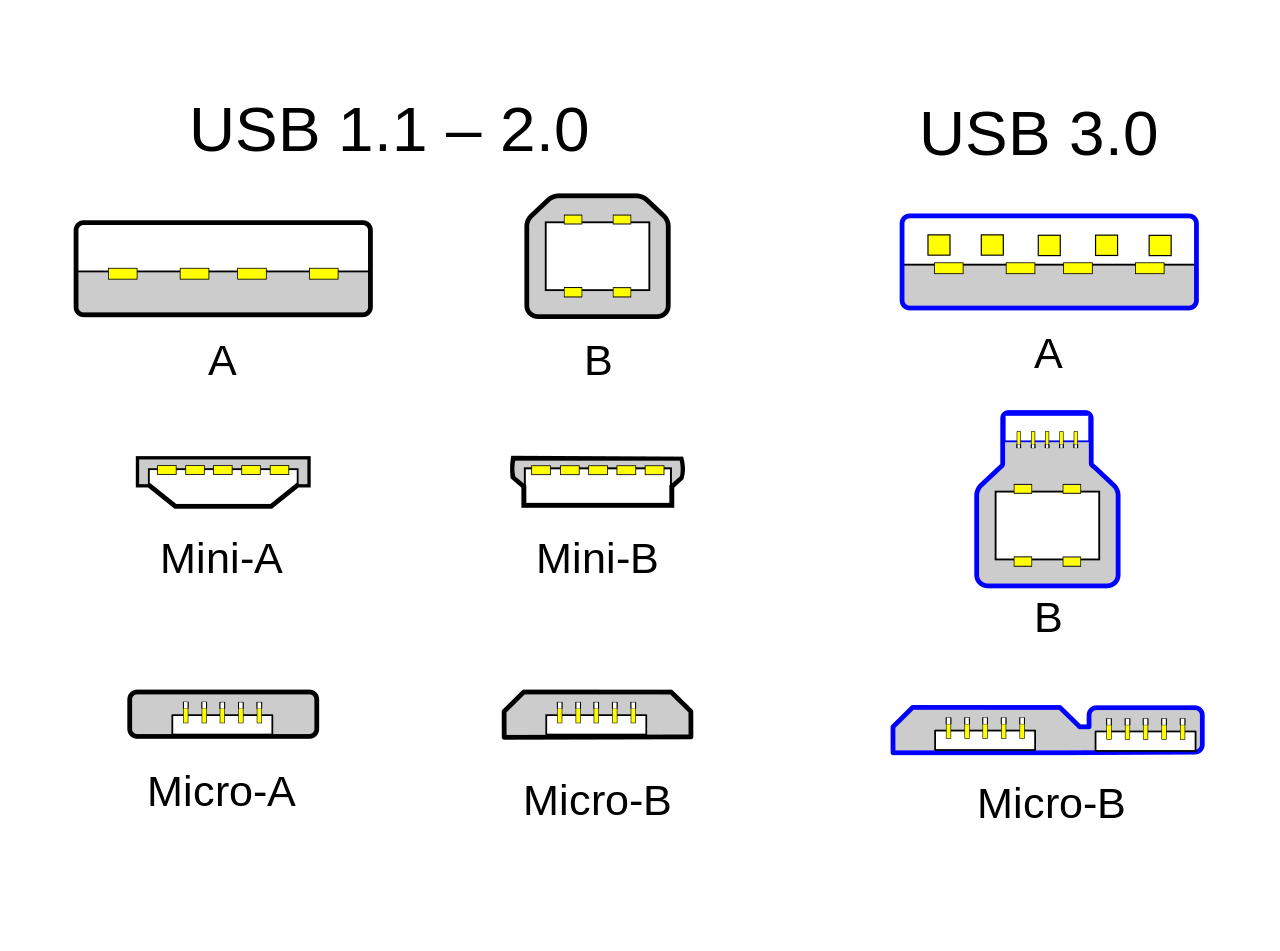
\includegraphics[width=0.4\textwidth]{images/usb_connectors.png}
    \caption{Connectors USB de tipus A i B. \cite{Contributors2024USB}}
    \label{fig:usb_connectors}
\end{figure}

\begin{itemize}
    \item Els connectors de tiups A son els que es connecten al dispositiu
    que actuarà com a mestre. Existeixen les variants \est{micro} i \est{mini},
    com es pot observar a la Figura \ref{fig:usb_connectors}, tot i que aquestes
    so son gaire populars. Amb l'aparició de l'estàndard \acro{usb3}, es van
    dissenyar nous connectors que fóssin compatibles amb els dels estàndards
    anteriors.
    \item Els connectors de tipus B son els que es connecten a l'esclau. Aquests
    també tenen les variants \est{micro} i \est{mini}, molt utilitzades
    en l'electrònica domèstica. També es va crear nous connectors de tipus B
    per a poder acollir l'estàndard \acro{usb3}.
    \item Finalment, els connectors de tipus C no tenen una jerarquia definida:
    serveixen per a dispositius que poden ser mestres o esclaus en diferents
    moments donats. La decisió de qui actua de mestre es pacta just a l'inici
    de la connexió, mitjançant un protocol específic \cite{Axelson2015USB}.
    Aquest connector, a diferència de la reta, és reversible: es pot connectar
    en les dues orientacions possibles. Es pot veure l'aspecte del connector
    a la Figura \ref{fig:usb_connectors_c}.
\end{itemize}

\begin{figure}[ht]
    \centering
    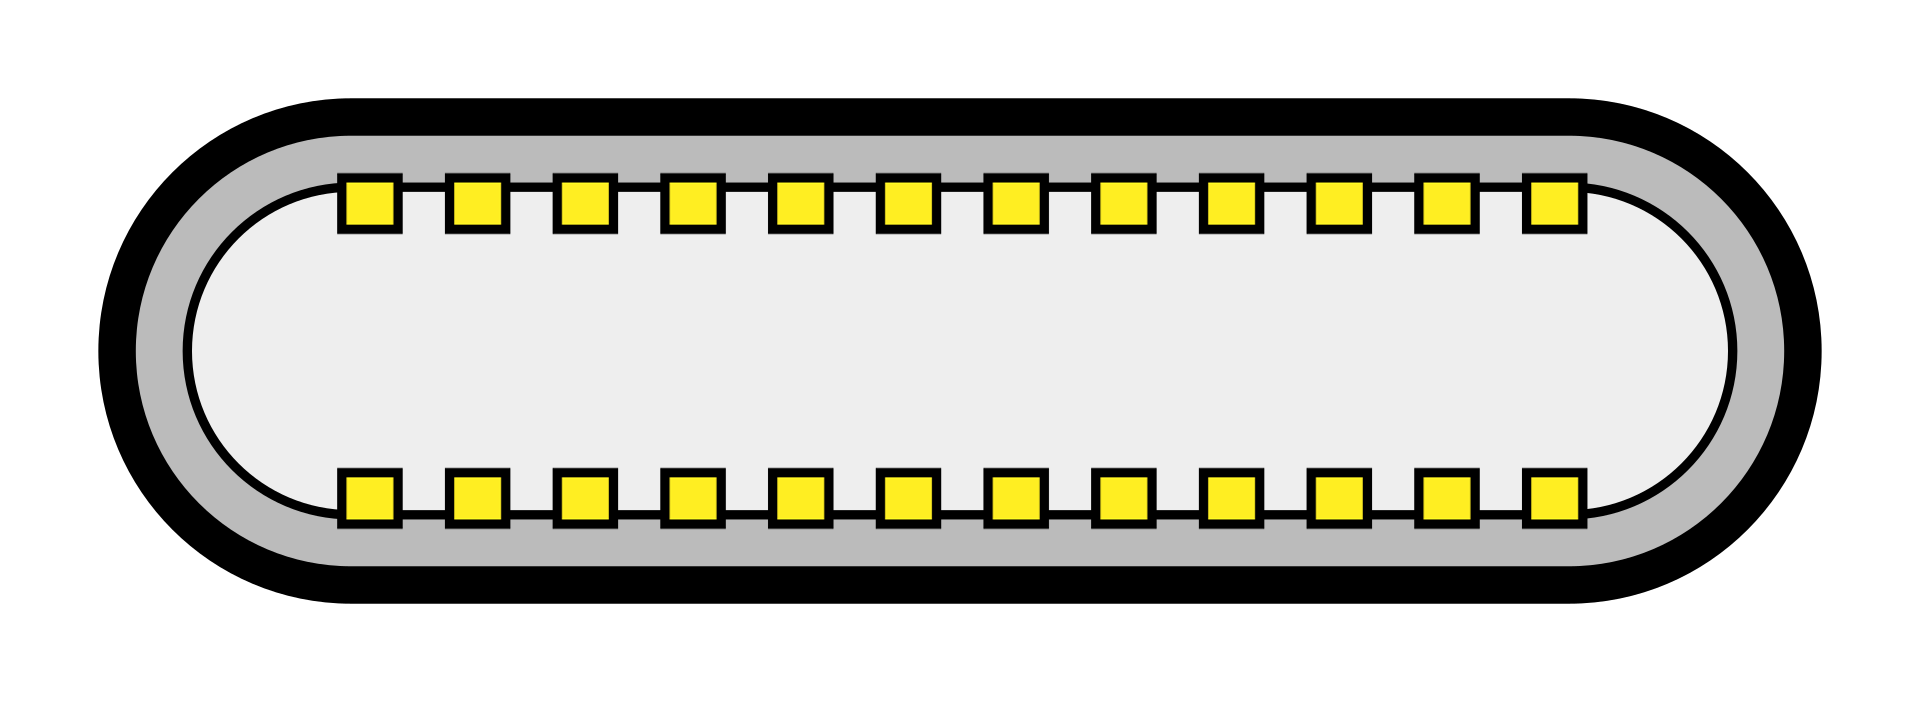
\includegraphics[width=0.2\textwidth]{images/usb_c.png}
    \caption{Connector USB de tipus C. \cite{Contributors2024USB}}
    \label{fig:usb_connectors_c}
\end{figure}

Així doncs, gairebé la totalitat de cables \acro{usb} seran de tipus A a tipus
B, utilitzant qualsevol format de mida. El tipus C, al ser bidireccional, pot
substituir el tipus A o el tipus B en els cables mencionats anteriorment.
Quan un cable només té un connector de tipus C en un cantó, no s'ha de pactar
la jerarquia de mestre-esclau, ja que ve definida pel tipus de connector a
l'altra banda del cable. Evidentment, també hi pot haver cables de tipus C a
tipus C.

Tanmateix, a l'any 2022 el Consell de la Unió Europea va aprovar una llei
que obliga un seguit de dispositius electrònics a utilitzar el connector
\acro{usb-c} enlloc d'altres estàndards \cite{Council2022Common}. Segons la
nota de premsa, el motiu d'aquesta llei és per a evitar més deixalla electrònica
per culpa de tenir diferents dispositius amb diferents connectors, així com
facilitar l'ús de les tecnologies als consumidors. Aquesta llei
es començarà a aplicar a finals de l'any 2024, i afectarà dispositius mòbils, 
alguns portàtils, tauletes, teclats i ratolins ina\l.làmbrics, entre
d'altres.

Sent el dispositu que es vol crear en aquest projecte un perifèric de
l'ordinador, la llei citada no l'afectaria. Tanmateix, la mateixa nota de premsa
informa sobre la intenció d'extendre aquest connector a altres dispositius.
Tenint present que el dispositiu que es vol crear podria entrar fàcilment en
aquest grup de perifèrics d'ordinador, s'ha decidit utilitzar un connector de
tipus \acro{usb-c} per a assegurar-nos la seva possible comercialització dintre
de la \acro{UE}.


\section{\est{Drivers} a Linux}

Un altre dels aspectes importants del projecte és la creació d'un programari
que pugui fer d'intermediari entre el dispositiu i l'entorn gràfic. Tal i com
diu el títol de l'apartat, es comentarà només el cas específic dels sistemes
\acro{UNIX}, concretament amb Linux.
